
\chapter{Cumulative Surface Deformation over the Permian Basin with Automated Outlier Removal}
\label{CHAP:4-GRL}

\section{Introduction}


%In this chapter,  we present a simple yet effective time series method for creating cumulative surface deformation maps over large regions with severe tropospheric noise. We use the method to create yearly deformation maps over the oil-producing region of the Permian Basin. The method incorporates an automated outlier detection and removal algorithm, which enabled ~2 mm/year agreement with GPS measurements in the presence of $\sim$15 cm of tropospheric noise.


In this chapter,  we present a time series method for creating large cumulative surface deformation maps over areas containing severe tropospheric noise. The method detects noise outliers withing multiple subsets of interferograms and produces a linear velocity estimate for each subset.  We use the method to create yearly deformation maps over the oil-producing region of the Permian Basin which agree with GPS measurements within ~2 mm/year.



Within Texas, \cite{Shirzaei2016SurfaceUpliftTime} reported indications of surface uplift due to wastewater injection near a 2012 M4.8 earthquake, though limited validation for the ALOS data was available at this site near Timpson, TX \citep{Semple2017IncompleteInventorySuspected}. \cite{Kim2018AssociationLocalizedGeohazards} detected multiple deformation bowls within the Delaware Basin related to wastewater injection, $CO_2$ injection, and hydrocarbon production using Sentinel-1 InSAR data. \cite{Zheng2019WastewaterLeakageWest} incorporated InSAR-derived surface deformation data into a poroelastic model to analyze the geomechanical processes near an uplift signal in northern West Texas. They discovered that the observed surface deformation was likely caused by injection well leakages, rather than pressure increases at the planned injection depth, and the leaks may have contributed to freshwater contamination. More recently, \cite{Deng2020SurfaceDeformationInduced} used ascending Sentinel-1 LOS measurements to infer pore pressure change and Coulomb failure stress change at three sites in the southern Delaware Basin. They suggested that certain groups of earthquakes are likely induced by fluid injection, but noted that local rock structure and media properties are key controls on the area's susceptibility to induced seismicity.

Previous InSAR studies demonstrated the use of InSAR surface deformation data for understanding causes of induced seismicity; however, these studies only focused on study areas $ \sim $ 60-by-60km or smaller, and basin-wide InSAR surface deformation data with detailed uncertainty quantification are needed for assessing the likelihood of induced seismicity risk. Since InSAR tropospheric noise variance increases with the distance away from the reference point \citep{Emardson2003NeutralAtmosphericDelay}, it is difficult to expand the InSAR spatial coverage to the entire Permian basin while retaining millimeter level accuracy. 

In this chapter, we show that the increasing quantity and quality of Sentinel-1 SAR data allows us to average thousands of interferograms and mitigate strong tropospheric noise. Additionally, we developed an outlier detection algorithm that removes InSAR measurements corrupted by severe tropospheric noise (e.g. storms and heat waves) and reduces InSAR measurement uncertainty by another factor of 2, down to 1-3 mm/year across the basin. Our results were validated by independent GPS measurements recorded at 13 permanent ground stations. The InSAR-observed subsidence patterns over the Pecos area can be modeled as dip-slip over multiple normal faults and discretized cylindrical reservoir compaction. Our InSAR deformation maps are now available through the Center for Integrated Seismicity Research (CISR) for the broader scientific community. This dataset, when combined with physics-based reservoir and fault modeling, can produce insights into the causes of induced seismicity. Furthermore, these surface deformation data products can be used to assess the areal effectiveness of the oil and gas production, a measure for estimating which regions of a reservoir are being depleted most quickly. InSAR techniques now provide a low-cost method to assist oil and gas operations and risk management at a basin-scale.

\section{Methods}
\subsection{InSAR data processing strategy}
\label{sec:InSARprocessing}
Using a geocoded SLC processor \citep{Zheng2017PhaseCorrectionSingle, Zebker2017UserFriendlyInsar}, we processed 91 ascending (path 78, frames 94-104) and 82 descending (path 85, frames 483-493) Sentinel-1 scenes acquired between Nov. 2014 and Jan. 2019 (Figure \ref{fig:paper1-study-area}). We generated more than 7000 interferograms with 120 meter pixel spacing and a maximum temporal baseline of 800 days. No spatial baseline threshold was imposed in the interferogram formation. Because few decorrelation artifacts were presented, we were able to unwrap all interferograms without additional spatial filtering using the Statistical-cost, Network-flow Algorithm for Phase Unwrapping (SNAPHU) \citep{Chen2001TwoDimensionalPhase}. We removed long-wavelength phase ramps, possibly due to residual orbit errors or long-wavelength tropospheric noise, using a planar phase model. Comparable interferograms can be generated using other processors such as the InSAR Scientific Computing Environment (ISCE) \citep{Rosen2012InsarScientificComputing}. 


\begin{figure}[hbt!]
	\centering
	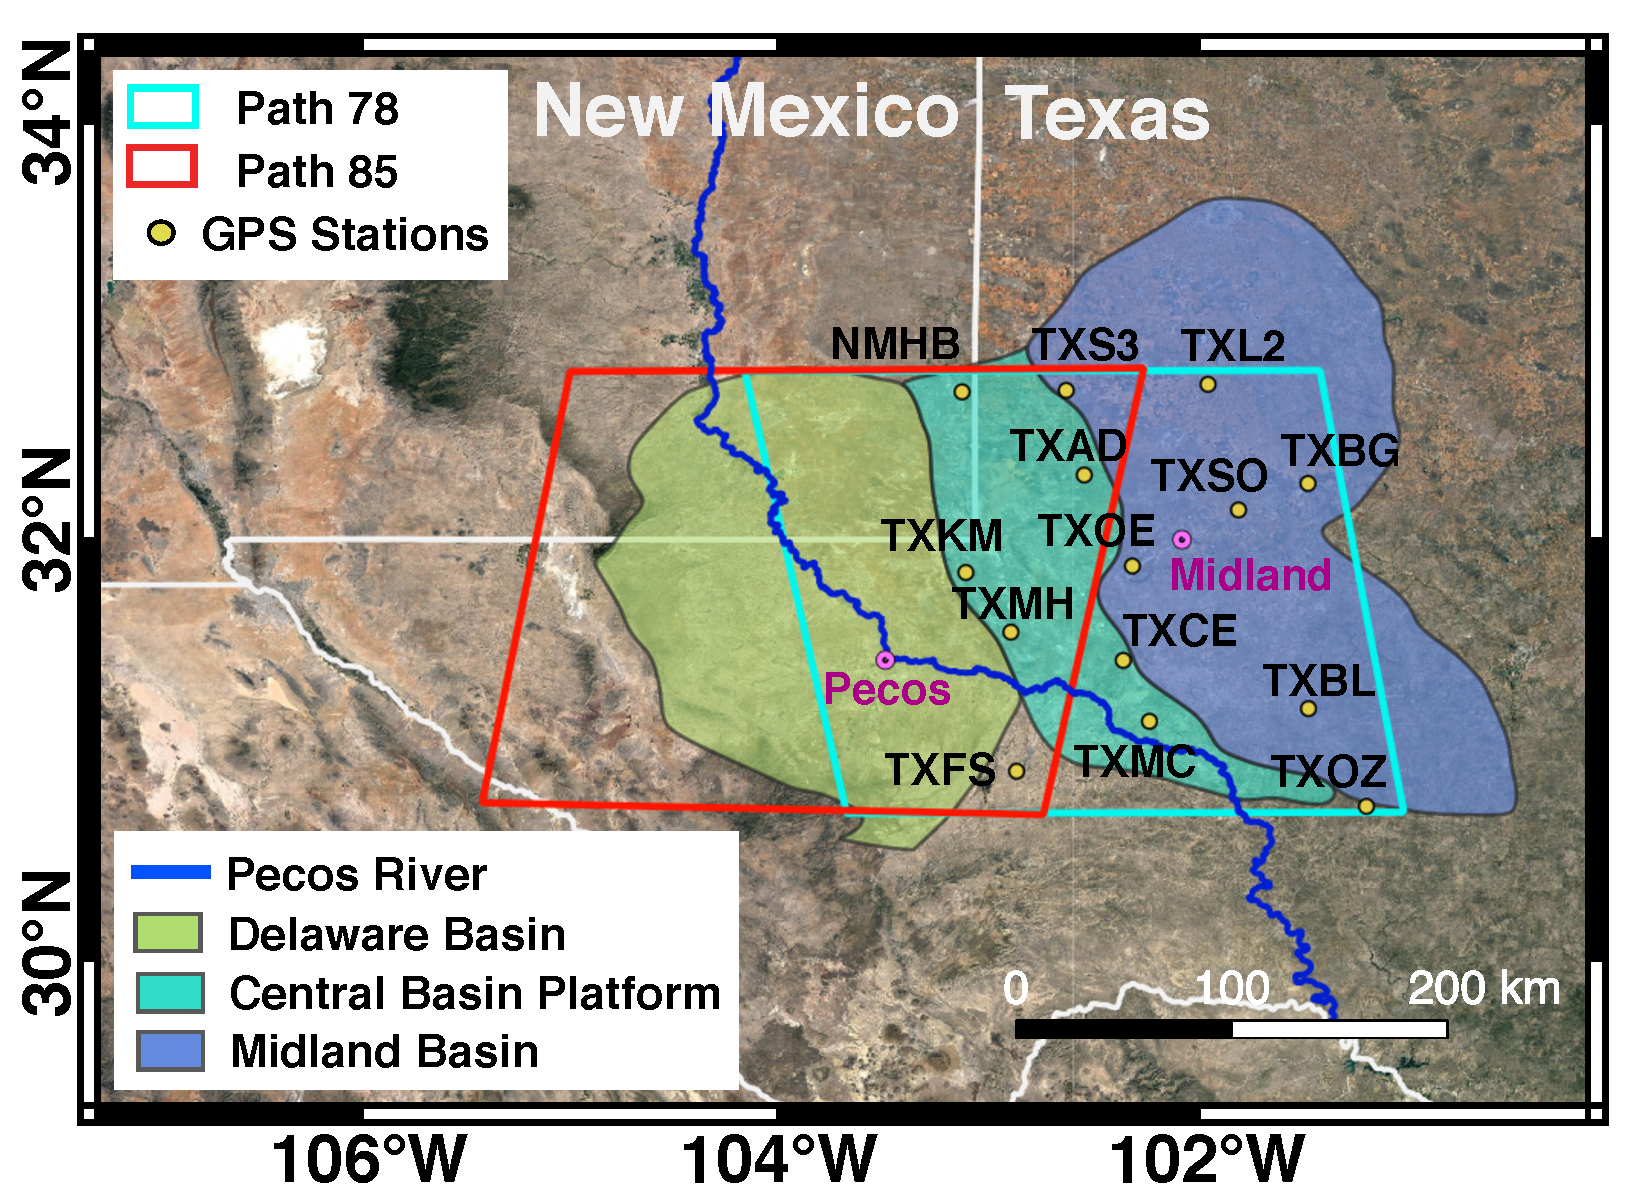
\includegraphics[width=0.9\linewidth]{paper1-permian/figures/figure1-study-area.pdf}
	\caption[GPS and InSAR data coverage over the Permian Basin.]{GPS and InSAR data coverage over the Permian Basin. Yellow dots indicate GPS permanent stations. Teal and red boxes indicate ascending path 78 and descending path 85 paths of Sentinel 1 InSAR coverage, respectively. Each path contains over 80 SAR acquisitions, leading to over 3500 interferograms per path at 120 m pixel spacing.}
	\label{fig:paper1-study-area}
\end{figure}


The coverage of GPS permanent stations in West Texas is sparse, and there are 14 permanent GPS stations (Figure \ref{fig:paper1-study-area}) that recorded daily east, north, and up (ENU) surface deformation measurements \citep{Blewitt2018HarnessingGpsData}. After removing the common tectonic motion, all GPS stations showed little surface deformation (0-3 mm/year) between Nov. 2014 and Jan. 2019. We chose the GPS station TXKM as the reference point for both ascending and descending InSAR data, and we used the remaining 13 stations as controls to assess InSAR measurement uncertainty as described in Section \ref{sec:errors}.

\subsection{Solutions for cumulative surface deformation over time}
\label{sec:stacking}
An interferogram measures surface deformation that occurred between the two SAR acquisition times along the radar line-of-sight (LOS) direction \citep{Hanssen2001RadarInterferometryData}. We employed a stacking approach \citep{Sandwell1998PhaseGradientApproach} to calculate the average LOS velocity $v_{avg}$ of each ground pixel over a time period of interest $T$ as:
\begin{equation}
	v_{avg} = \frac{\sum_{i \in G} d_i}{\sum_{i \in G} t_i}
	\label{eq:stacking}
\end{equation}
where $G$ is a subset of interferograms that were formed using two SAR scenes acquired within the time period $T$. The LOS measurement (in cm) and the temporal baseline of the $i^{th}$ interferogram in $G$ are written as $d_i$ and $ t_i $ respectively. In Section \ref{sec:method-compare}, we show that comparable LOS velocity estimates can be produced using the Small Baseline Subset (SBAS) approach \citep{Berardino2002NewAlgorithmSurface} with a constant velocity (linear deformation) model.

In this study, we solved for the average LOS velocities over three periods of interest: Nov. 2014 to Jan. 2017, Nov. 2014 to Jan. 2018, and Nov. 2014 to Jan. 2019. Over each period $T_j$, we computed the cumulative LOS surface deformation over this period as the product of $v_{avg,j}$ and $T_j$. We also solved for the vertical and eastward deformation in the region where path 78 and 85 overlap ( \textit{Supporting Information S2}). To account for the large variation in look angle within one Sentinel-1 Interferometric Wide (IW) swath image, we used the LOS unit vector at each pixel location Figure \ref{fig:los-map})) in the LOS decomposition.


\subsection{A comparison between stacking and InSAR time series methods}
\label{sec:method-compare}
%If data error treatments and deformation model assumptions are valid, we can derive meaningful and comparable deformation solutions using different InSAR time series analysis methods. 
To investigate how InSAR measurement noise influences the LOS deformation solutions, we compared the results derived from (1) the stacking method, (2) a Small BAseline Subset (SBAS) linear deformation (constant velocity) model with $L_1$ and $L_2$-norm penalty functions, and (3) unregularized and regularized SBAS deformation time series. 

For the remainder of this section, we assume there are $M$ small-baseline interferograms that were generated from $N$ SAR scenes acquired over a period of interest. The stacking method from \cite{Sandwell1998PhaseGradientApproach} that we employed in this study solves for the average velocity over the study period. Similarly, the SBAS linear deformation model solves for the average velocity $ v_{avg} $ over this period at each pixel of interest as \citep{Berardino2002NewAlgorithmSurface}:
\begin{equation}
	\arg \min_{v_{avg}} \norm{ \bm{BP} v_{avg} - \bm{d}   }_p
	\label{eq:sbas-linear}
\end{equation}
where $ \bm{B }$ is the $ M \times (N-1) $ SBAS matrix, $ \bm{P}$ is an $ (N-1) \times 1 $ vector of ones, $ \bm{d} $ is the $ M \times 1 $ vector of LOS measurements (in cm) at this pixel, and $ p \in \{1, 2\} $ is the norm used to penalize the data misfit. The $L_2$ linear deformation solution is comparable to the stacking solution (with an assumption of a constant velocity), and the $L_1$ solution is typically less sensitive to measurement outliers than the $L_2$ solution.

The LOS surface velocities between adjacent SAR acquisitions $ \bm{v} = \left[v_1 , \ldots , v_{N-1} \right]^T $ can be solved as:
\begin{equation}
	\arg \min_{\bm{v} } \norm{ \bm{Bv} - \bm{d}   }^2_2 + \alpha \norm{ \bm{Dv} }^2_2  \label{eq:sbas}
\end{equation}
where $ \bm{D} $ is a $ (N-2) \times (N-1) $ matrix, with $1$ on the main diagonal and $-1$ on the superdiagonal, which approximates the first-order differentiation operator. The first term penalizes the data misfit, the second term is a temporal smoothness constraint, and $ \alpha \in \mathbb{R} $ is the weight between the two terms. When $ \alpha = 0 $, the solution is the unregularized SBAS deformation time series. An additional integration of $\mathbf{v}$ over time yields the LOS deformation time series.

Little surface deformation occurred between Nov. 2014 and Jan. 2019 at the 13 GPS permanent GPS stations. At each GPS location, we projected the GPS time series to the radar line-of-sight (LOS), and we used the GPS-inferred average LOS velocity (0-3 mm/year) as ground truth. Table \ref{tab:compare-errors} shows the root mean square (RMS) and the worst-case absolute differences between InSAR and GPS inferred average LOS velocities between Nov. 2014 and Jan. 2018 as derived from the four InSAR time series methods. We found that InSAR tropospheric noise has a strong influence on all the surface deformation solutions before removing the measurement outliers. As an example, Figure \ref{fig:compare} (a) shows the ascending LOS solutions between Nov. 2014 and Jan. 2018 at the GPS station TXSO before removing InSAR measurement outliers. The random tropospheric noise creates up to $\sim$6 cm of error in the unregularized SBAS surface deformation time series. This error can be reduced by increasing $ \alpha$ in Equation \eqref{eq:sbas}. As $\alpha$ increases, the LOS deformation time series converge to the $L_2$ linear deformation (constant velocity) solution. However, there are visible cm-level tropospheric artifacts in the cumulative deformation solutions by using either $L_1$ or $L_2$ linear deformation models (e.g. Figure 2 (d) in the main text). 

After removing InSAR outlier measurements associated with extreme local weather events as described in Section 2.3 (main text), all SBAS time series methods produce more accurate and consistent deformation trends (Figure \ref{fig:compare} (b)). The unregularized SBAS time series still contain up to $\sim$3 cm of tropospheric noise, which leads to long-wavelength artifacts in the basin-wide deformation maps. The $ L_1 $ and $ L_2 $ linear deformation solutions show close agreement ($<$ 2 mm difference) at all GPS stations. Since both methods suggest a deformation trend consistent with the stacking approach, we chose the simple stacking method as the final processing strategy for estimating cumulative surface deformation in the Permian Basin.

\begin{figure}
	\centering
	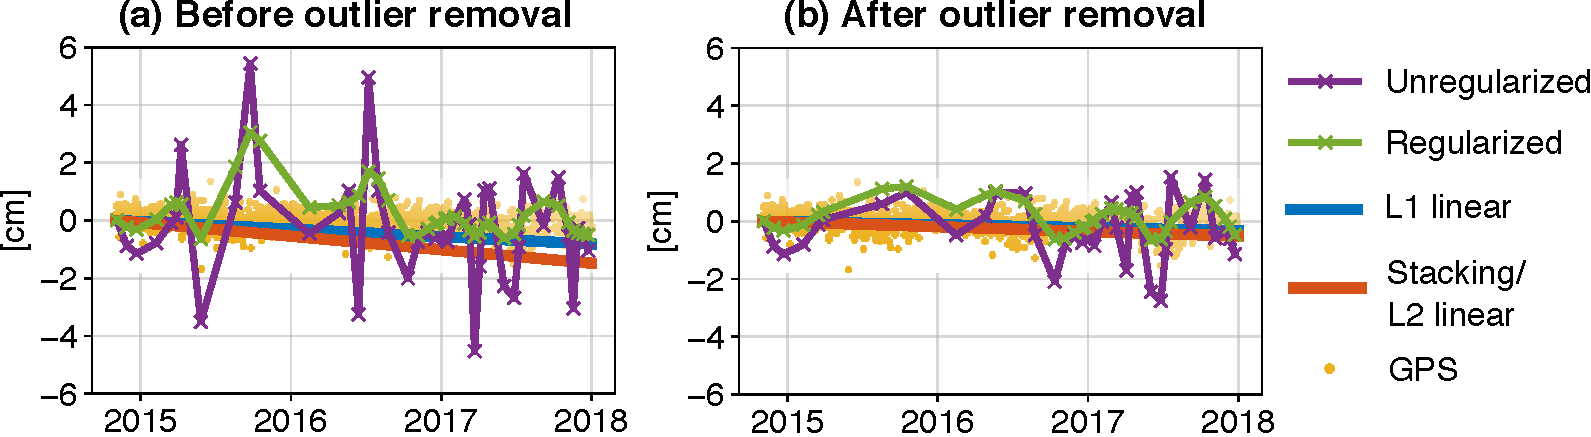
\includegraphics[width=\textwidth]{paper1-permian/figures/supplement/figureS5-compare-insar-2panel.pdf}
	\caption[Comparisons of InSAR SBAS solutions]{Comparisons of InSAR unregularized SBAS time series (purple), regularized SBAS time series (green), linear deformation trend estimated by minimizing the $L_1$-norm of the residuals (blue), and the $L_2$-norm of the residuals/ stacking approach (red)  (a) before and (b) after removing LOS measurement outliers. ENU GPS data from station TXSO has been projected onto the radar LOS (orange dots).}
	\label{fig:compare}
\end{figure}

\subsection{Errors in InSAR surface deformation estimates}
\label{sec:errors} 
As outlined in Section \ref{sec:ch3-noise}, the phase of an interferogram can be written as \citep{Zebker1992DecorrelationInterferometricRadar, Zebker1994AccuracyTopographicMaps, Zebker1997AtmosphericEffectsInterferometric}
\begin{equation}
	\Delta \phi = \frac{4 \pi}{\lambda} \Delta d_{LOS} +  \Delta \phi_{orb} + \Delta \phi_{decor} + \Delta \phi_{unwrap}  + \Delta \phi_{dem} + \Delta \phi_{iono} + \Delta \phi_{tropo}  + \Delta \phi_{n}
\end{equation}
where $ \lambda $ is the radar wavelength and $ \Delta d_{LOS} $ is the surface deformation along the radar LOS direction. The noise terms include orbital errors, phase decorrelation, unwrapping errors, DEM inaccuracies, ionospheric and tropospheric artifacts, and other residual noise terms that are typically an order of magnitude smaller than the error terms listed here. Following the processing strategy outlined in Section \ref{sec:InSARprocessing}, $\Delta \phi_{orb}$, $\Delta \phi_{decor}$, and $\Delta \phi_{unwrap}$ were either removed or negligible in our dataset. Because the relatively flat Permian Basin is located in the middle latitudes, $\Delta \phi_{dem}$ and $\Delta \phi_{iono}$ are not substantial \citep{Fattahi2013DemErrorCorrection, Liang2019IonosphericCorrectionInsar}. For the reminder of this section, we focused on evaluating and mitigating the impact of tropospheric noise on the West Texas Sentinel-1 data.


%
%\subsection{The impact of the stratified component of tropospheric noise}
%\label{sec:noise-quant}


As described in Chapter \ref{sec:ch3-noise-tropo}, tropospheric noise $\Delta \phi_{tropo}$ consists of a stratified component that correlates with topography \citep{Doin2009CorrectionsStratifiedTropospheric} and a turbulent component that is random at time scales longer than one day \citep{Emardson2003NeutralAtmosphericDelay}. We checked for a stratified tropospheric noise component using the Generic Atmospheric Correction Online Service (GACOS), and we found that the stratified tropospheric errors in our Sentinel-1 data are minimal. This is because the oil-producing region of the Permian Basin is relatively flat, and we observed little correlation between InSAR LOS measurements and the Digital Elevation Model (DEM) data (e.g. Figure \ref{fig:GACOS} (d)). 



We further examined interferograms at the 13 control locations. For example, LOS measurements of the ascending interferograms at pixels near the GPS station TXMC show a near zero median (-4 mm) and a standard deviation of 3.2 cm (Figure \ref{fig:outliers} (a)). Due to the absence of substantial deformation signal at this station, the standard deviation of the LOS distribution is a measure of turbulent tropospheric noise.  We found that the median LOS turbulent error is close to zero (no systematic noise bias) at all GPS control stations. The standard deviation of the turbulent noise increases as the square root of the distance from the InSAR reference point (Figure \ref{fig:outliers} (b)). Furthermore, we compared the LOS turbulent noise distribution observed at each GPS station to a normal distribution using a normal probability plot \citep{Filliben1975ProbabilityPlotCorrelation}. We discovered that non-Gaussian tails (outliers) are present (e.g. Figure \ref{fig:outliers}(c)) as a result of severe tropospheric noise (e.g. storms or heat waves). Identifying and removing these InSAR measurement outliers is crucial for achieving millimeter level accuracy. 




\begin{figure}[hbt!]
	\centering
	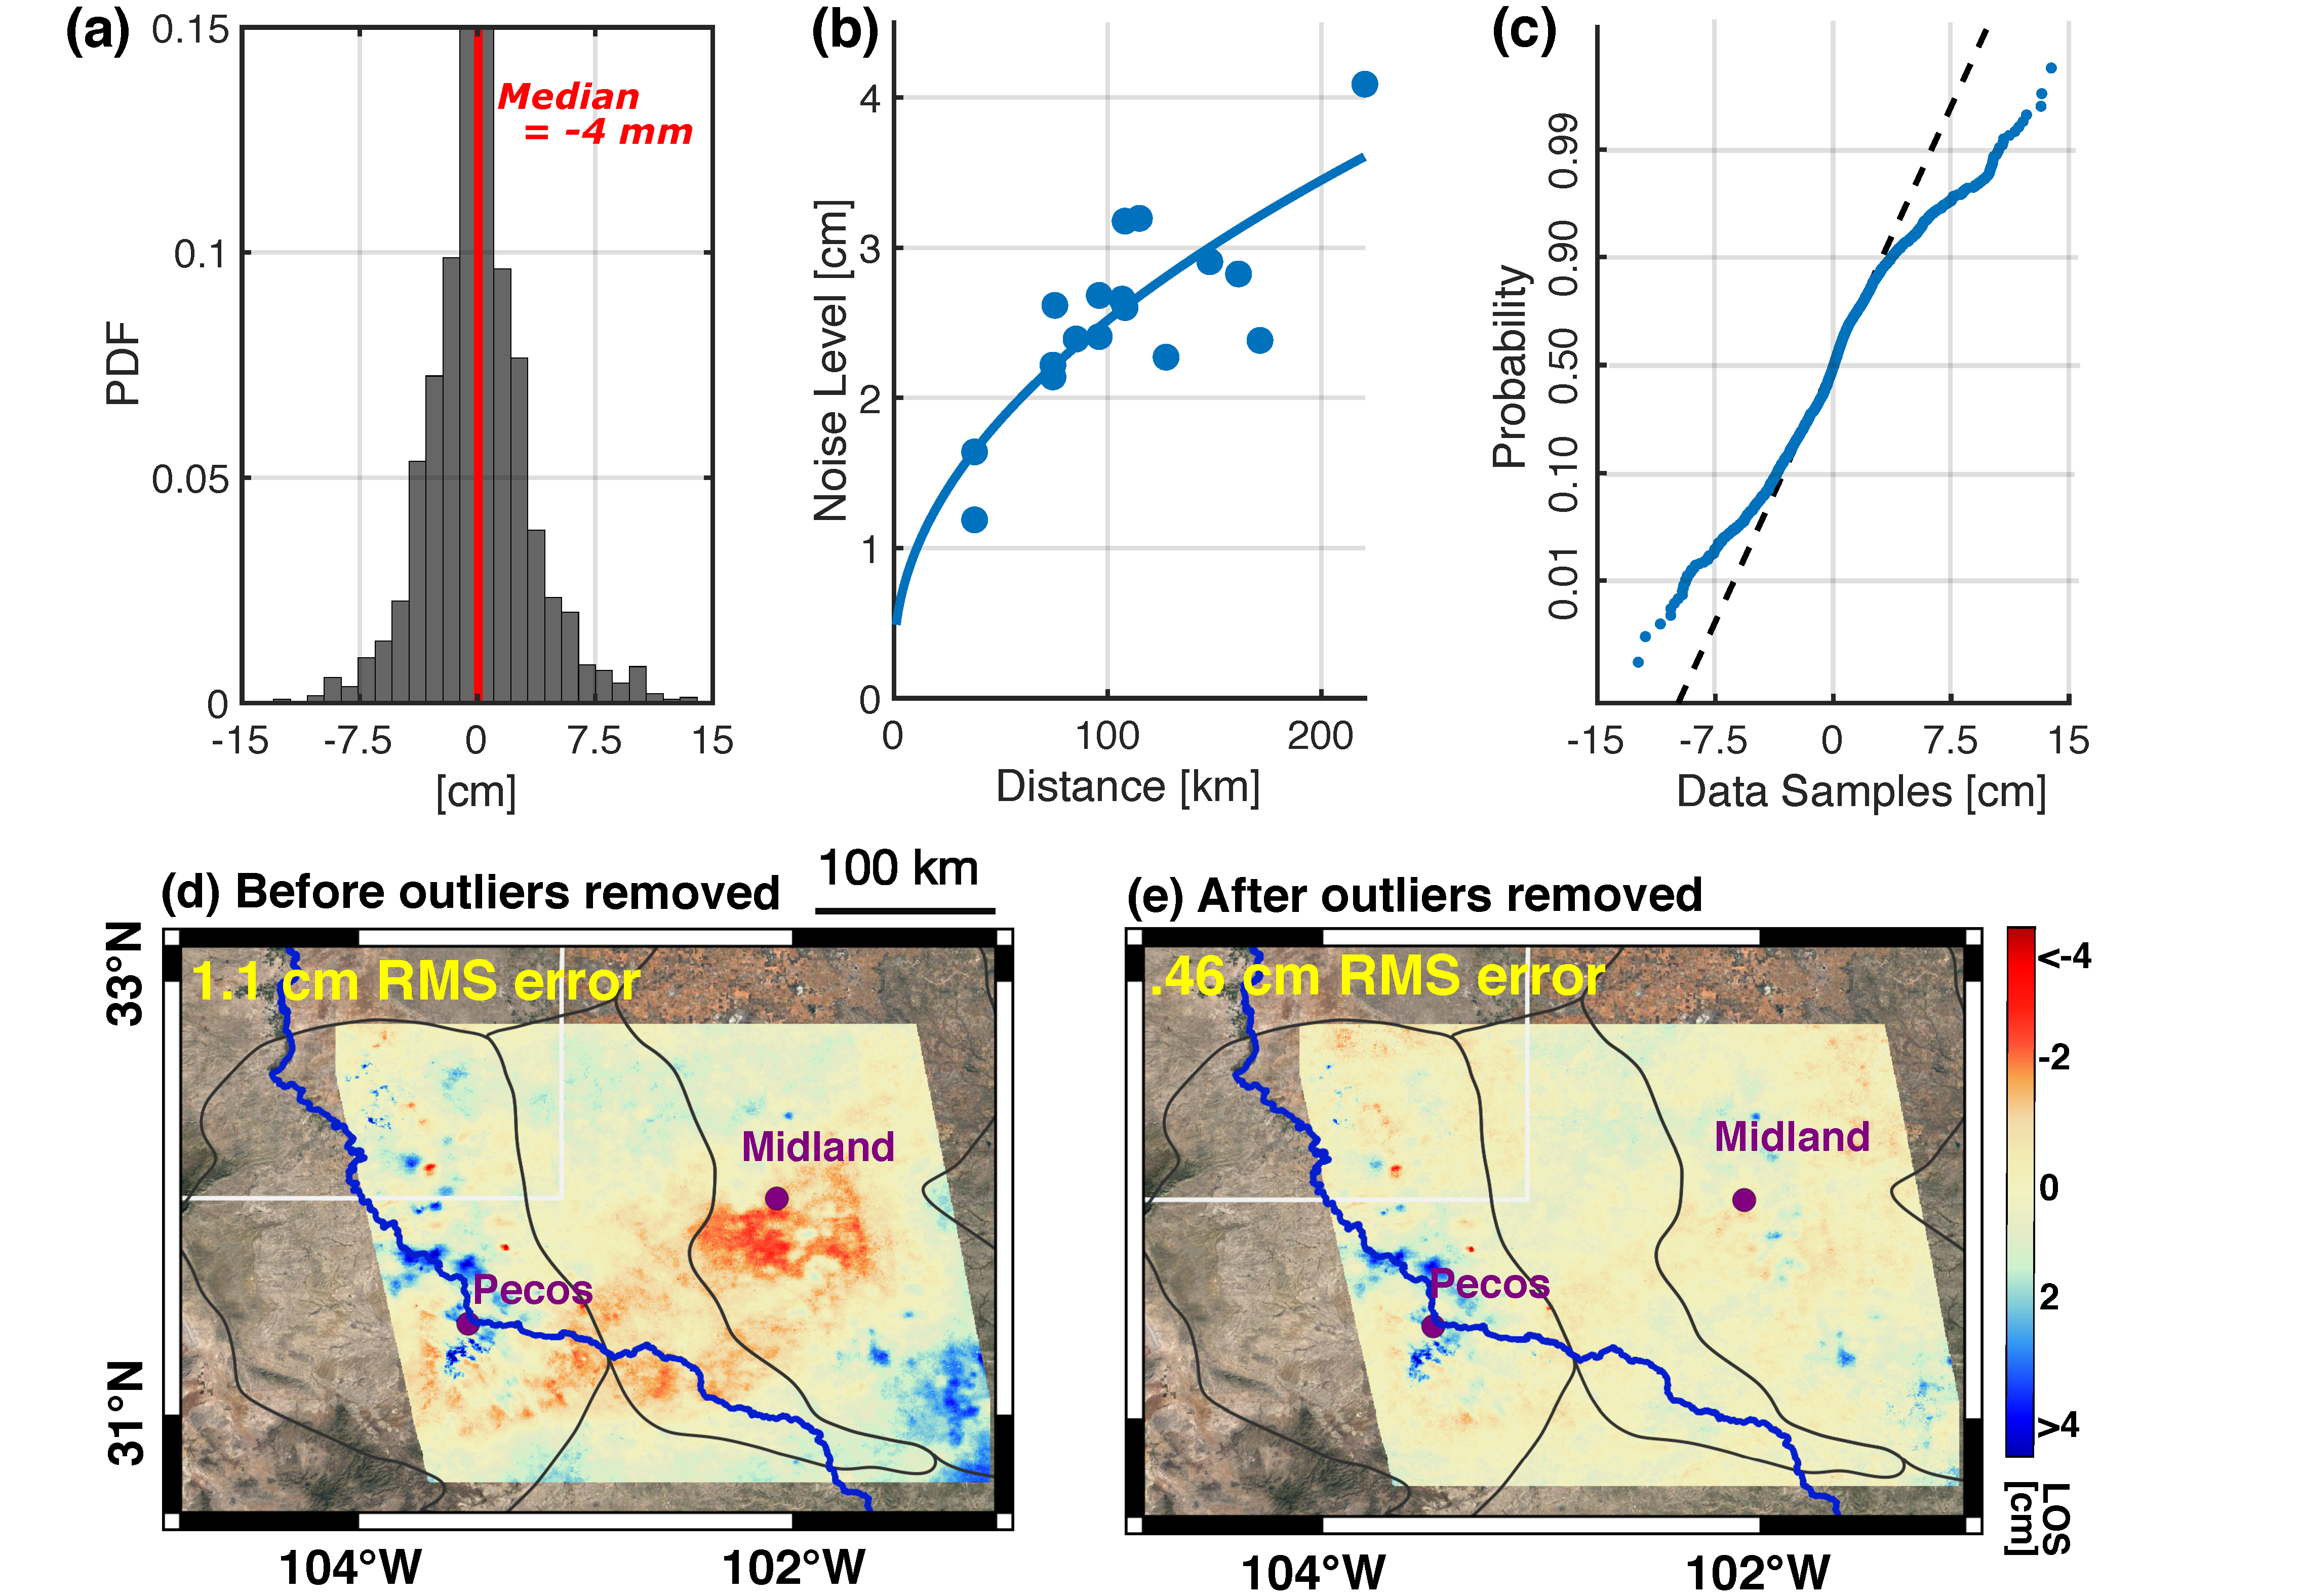
\includegraphics[width=0.95\linewidth]{paper1-permian/figures/figure2-outlier-removal-5panel.pdf}
	\caption[Noise measurement and tropospheric outlier removal comparison]{(a) LOS measurements (in cm) of all ascending interferograms at the GPS station TXMC. The distribution has a near zero median (-4 mm) and a standard deviation of 3.2 cm. Due to the absence of substantial deformation signals, the standard deviation of the distribution is a measure of LOS turbulent tropospheric noise. (b) The standard deviation of random tropospheric turbulent noise at 13 control locations (blue dots), which increases as the square root of the distance from the InSAR reference point (blue line). (c) A comparison between the tropospheric noise distribution at TXMC with a normal distribution. Dashed line connects the 1st and 3rd quartiles of the data. Troposphere noise following a normal distribution would match the dashed line, and non-Gaussian tails (we noted as outliers) are present. Cumulative ascending LOS deformation solutions (Nov. 2014 - Dec. 2017) (d) before and (e) after excluding InSAR outlier measurements. Note that 1.1 cm cumulative error over 3 years is equivalent to 3.5 mm/year RMS error in the velocity estimate.}
	\label{fig:outliers}
\end{figure}


Because severe tropospheric noise may only affect a portion of a SAR image, we identified InSAR measurement outliers at each pixel independently as follows. Given $N$ SAR acquisitions, there are up to $N-1$ InSAR LOS measurements at a pixel of interest that contain the common tropospheric noise of the $k^{th}$ SAR scene. We defined $u_{k,n}$ as the $n^{th}$ such LOS measurement, and $\bar{u}_k$ as:
\begin{equation}
	\bar{u}_k  = \frac{1}{N-1} \sum_{n=1}^{N-1} |u_{k,n}|  
\end{equation}
We labeled $u_{k,n}$ (for all $n$) as outlier measurements if $\bar{u}_k > \mathrm{median}(\mathbf{\bar{u}}) + 4 \sigma_{\mathrm{MAD}}$, where $\mathbf{\bar{u}}=[\bar{u}_1,...,\bar{u}_N]$, and $\sigma_{\mathrm{MAD}}=1.483 \cdot \mathrm{MAD}(\mathbf{\bar{u}})$. Here we employed a robust statistics measure, the median absolute deviation (MAD), for estimating the spread of data samples in the presence of outliers \cite{Hampel1974, Rousseeuw2011}. Given a vector $\mathbf{x}$ that contains $M$ data samples, $\mathrm{MAD}(\mathbf{x})$ is defined as:
\begin{equation}
	\mathrm{MAD}(\mathbf{x}) =  \underset{m = 1,\ldots M}{\mathrm{median}} \left( \bigr\lvert  x_m - \mathrm{median}(\mathbf{x})  \bigr\rvert \right)
\end{equation}
where $x_m$ is the $m^{th}$ data sample. 

To evaluate the performance of our InSAR processing strategy, we projected GPS data recorded at 13 control stations onto the LOS directions to use as ground truth. The differences between InSAR and GPS inferred average LOS velocities were used as a measure of the uncertainty in the InSAR surface deformation solutions (Section \ref{sec:error-quant}). We found that stacking reduces the impact of random Gaussian turbulent noise by $ \sim \sqrt{N} $, where $ N $ is the number of SAR acquisitions. The outlier removal algorithm further reduces the uncertainty in the LOS velocity estimates by a factor of 2, down to 1-3 mm/year across the basin. For example, the average InSAR velocity along the ascending LOS direction between Nov. 2014 and Jan. 2018 shows a root mean square (RMS) error of 3.4 mm/year before the outlier removal, and 1.5 mm/year after the outlier removal. The presence of InSAR measurement outliers resulted in long-wavelength artifacts ($ \sim $100km and greater) in the cumulative deformation solutions (e.g. Figure \ref{fig:outliers} (d)), which were automatically mitigated through the pixel-based outlier removal algorithm (e.g. Figure \ref{fig:outliers} (e)). Additionally, we compared InSAR LOS deformation solutions as derived from (1) the stacking method, (2) a SBAS linear deformation model with $L_1$ and $L_2$-norm penalty functions, and (3) unregularized and regularized SBAS deformation time series (\textit{Supporting Information S5}). These InSAR time series algorithms can be implemented using software packages such as Generic InSAR Analysis Toolbox (GIAnT) \citep{Agram2013NewRadarInterferometric}, STAMPS \citep{Hooper2012RecentAdvancesSar}, and LiCSBAS \citep{Morishita2020LicsbasOpenSource}. Removing the detected outliers leads to more accurate and consistent surface deformation solutions in all three cases.


\subsection{InSAR LOS velocity estimation errors using the stacking method}
\label{sec:error-quant}
We used independently processed GPS east, north, and up GPS time series as ground truth to quantify errors in the InSAR stacking solutions before and after the outlier removal. There are 13 permanent GPS stations in the ascending SAR footprint. At each GPS location, we projected the GPS time series to the radar line-of-sight (LOS), and we computed the GPS-inferred average LOS velocity through a linear regression. Table \ref{tab:gps-error-78} shows the root mean square (RMS) and the worst-case absolute differences between InSAR and GPS inferred average LOS velocities over the three study periods. Similarly, there are 5 permanent GPS stations in the descending SAR footprint, and Table \ref{tab:gps-error-85} shows the uncertainty in the descending stacking solutions using these 5 GPS stations as control. Both Table \ref{tab:gps-error-78} and Table \ref{tab:gps-error-85} show that our outlier removal algorithm reduced the uncertainty in InSAR stacking solutions by a factor of $\sim$2, down to 1-2 mm/year across the basin. For a given period of interest $T_j$, the LOS velocity error $ E_{vel,j} $ propagates into the cumulative deformation error $ E_{c, j} $ as $ E_{c,j} = E_{vel,j} \cdot T_j $. 


\begin{table}
	\caption{InSAR ascending LOS velocity estimation errors (in mm/year) using the stacking method}
	\centering
	\begin{tabular}{|c|c|c|}
		\hline 
		& Before the outlier removal & After the outlier removal \\
		& (RMS / Worst) & (RMS / Worst) \\
		\hline
		Nov. 2014 - Jan. 2017 & 3.8 / 9.5         & 1.9 / 5.9       \\\hline
		Nov. 2014 - Jan. 2018 & 3.3 / 7.1         & 1.3 / 2.5       \\\hline
		Nov. 2014 - Jan. 2019 & 2.0 / 6.1         & 1.1 / 2.5       \\\hline                
	\end{tabular}
	\label{tab:gps-error-78}
\end{table}

\begin{table}
	\caption{InSAR descending LOS velocity estimation errors (in mm/year) using the stacking method}
	\begin{tabular}{|c|c|c|}
		\hline 
		& Before the outlier removal & After the outlier removal \\
		& (RMS / Worst) & (RMS / Worst) \\
		\hline 
		Nov. 2014 - Jan. 2017 & 7.8 / 13.8                            & 2.9 / 5.0                          \\\hline
		Nov. 2014 - Jan. 2018 & 3.7 / 7.5                             & 2.7 / 5.6                          \\\hline
		Nov. 2014 - Jan. 2019 & 1.6 / 2.8                             & 0.8 / 1.6  \\\hline     
	\end{tabular}
	\label{tab:gps-error-85}
\end{table}

\begin{table}
	\caption{Errors (in mm) in four SBAS ascending LOS deformation (Nov. 2014 - Jan. 2018) solutions}
	\centering
	\begin{tabular}{|c|c|c|}
		\hline 
		& Before the outlier removal & After the outlier removal \\
		& (RMS / Worst) & (RMS / Worst) \\
		\hline
		Unregularized &  22 / 99     &  14 / 43         \\\hline
		Regularized   &    14 / 63   &   10  / 27       \\\hline
		L1 linear deformation          &   7 / 11      & 4 / 8      \\\hline
		L2 linear deformation          &   10 / 22        & 4 / 8      \\\hline
	\end{tabular}
	\label{tab:compare-errors}
\end{table}



\section{Results and discussion}
\subsection{Surface deformation in the Permian Basin}
The Sentinel-1 cumulative LOS deformation solutions reveal numerous surface deformation features over the oil-producing region in the Permian Basin (Figure \ref{fig:insar-los}). From the ascending geometry, we observed no substantial deformation in the Central Basin Platform, where oil and gas are mostly produced from conventional reservoirs. In the Midland and Delaware Basins, we observed an accelerating surface deformation rate between Nov. 2014 and Jan. 2019, which coincides with the sharp rise of oil production from unconventional reservoirs in 2017 and 2018. For example, a 30 km$^2 $ area northwest of Pecos shows approximately 0.5 cm cumulative LOS deformation between Nov. 2014 and Jan. 2017, 1.5 cm between Nov. 2014 and Jan. 2018, and over 5.5 cm from Nov. 2014 to Jan. 2019. The greatest number of observable signals are present in 2018 when peak production occurred in the region. Similarly, from the descending geometry, we find no substantial deformation in the Central Basin Platform and an increasing rate of surface deformation in the Delaware Basin. 


\begin{figure}[hbt!]
	\centering
	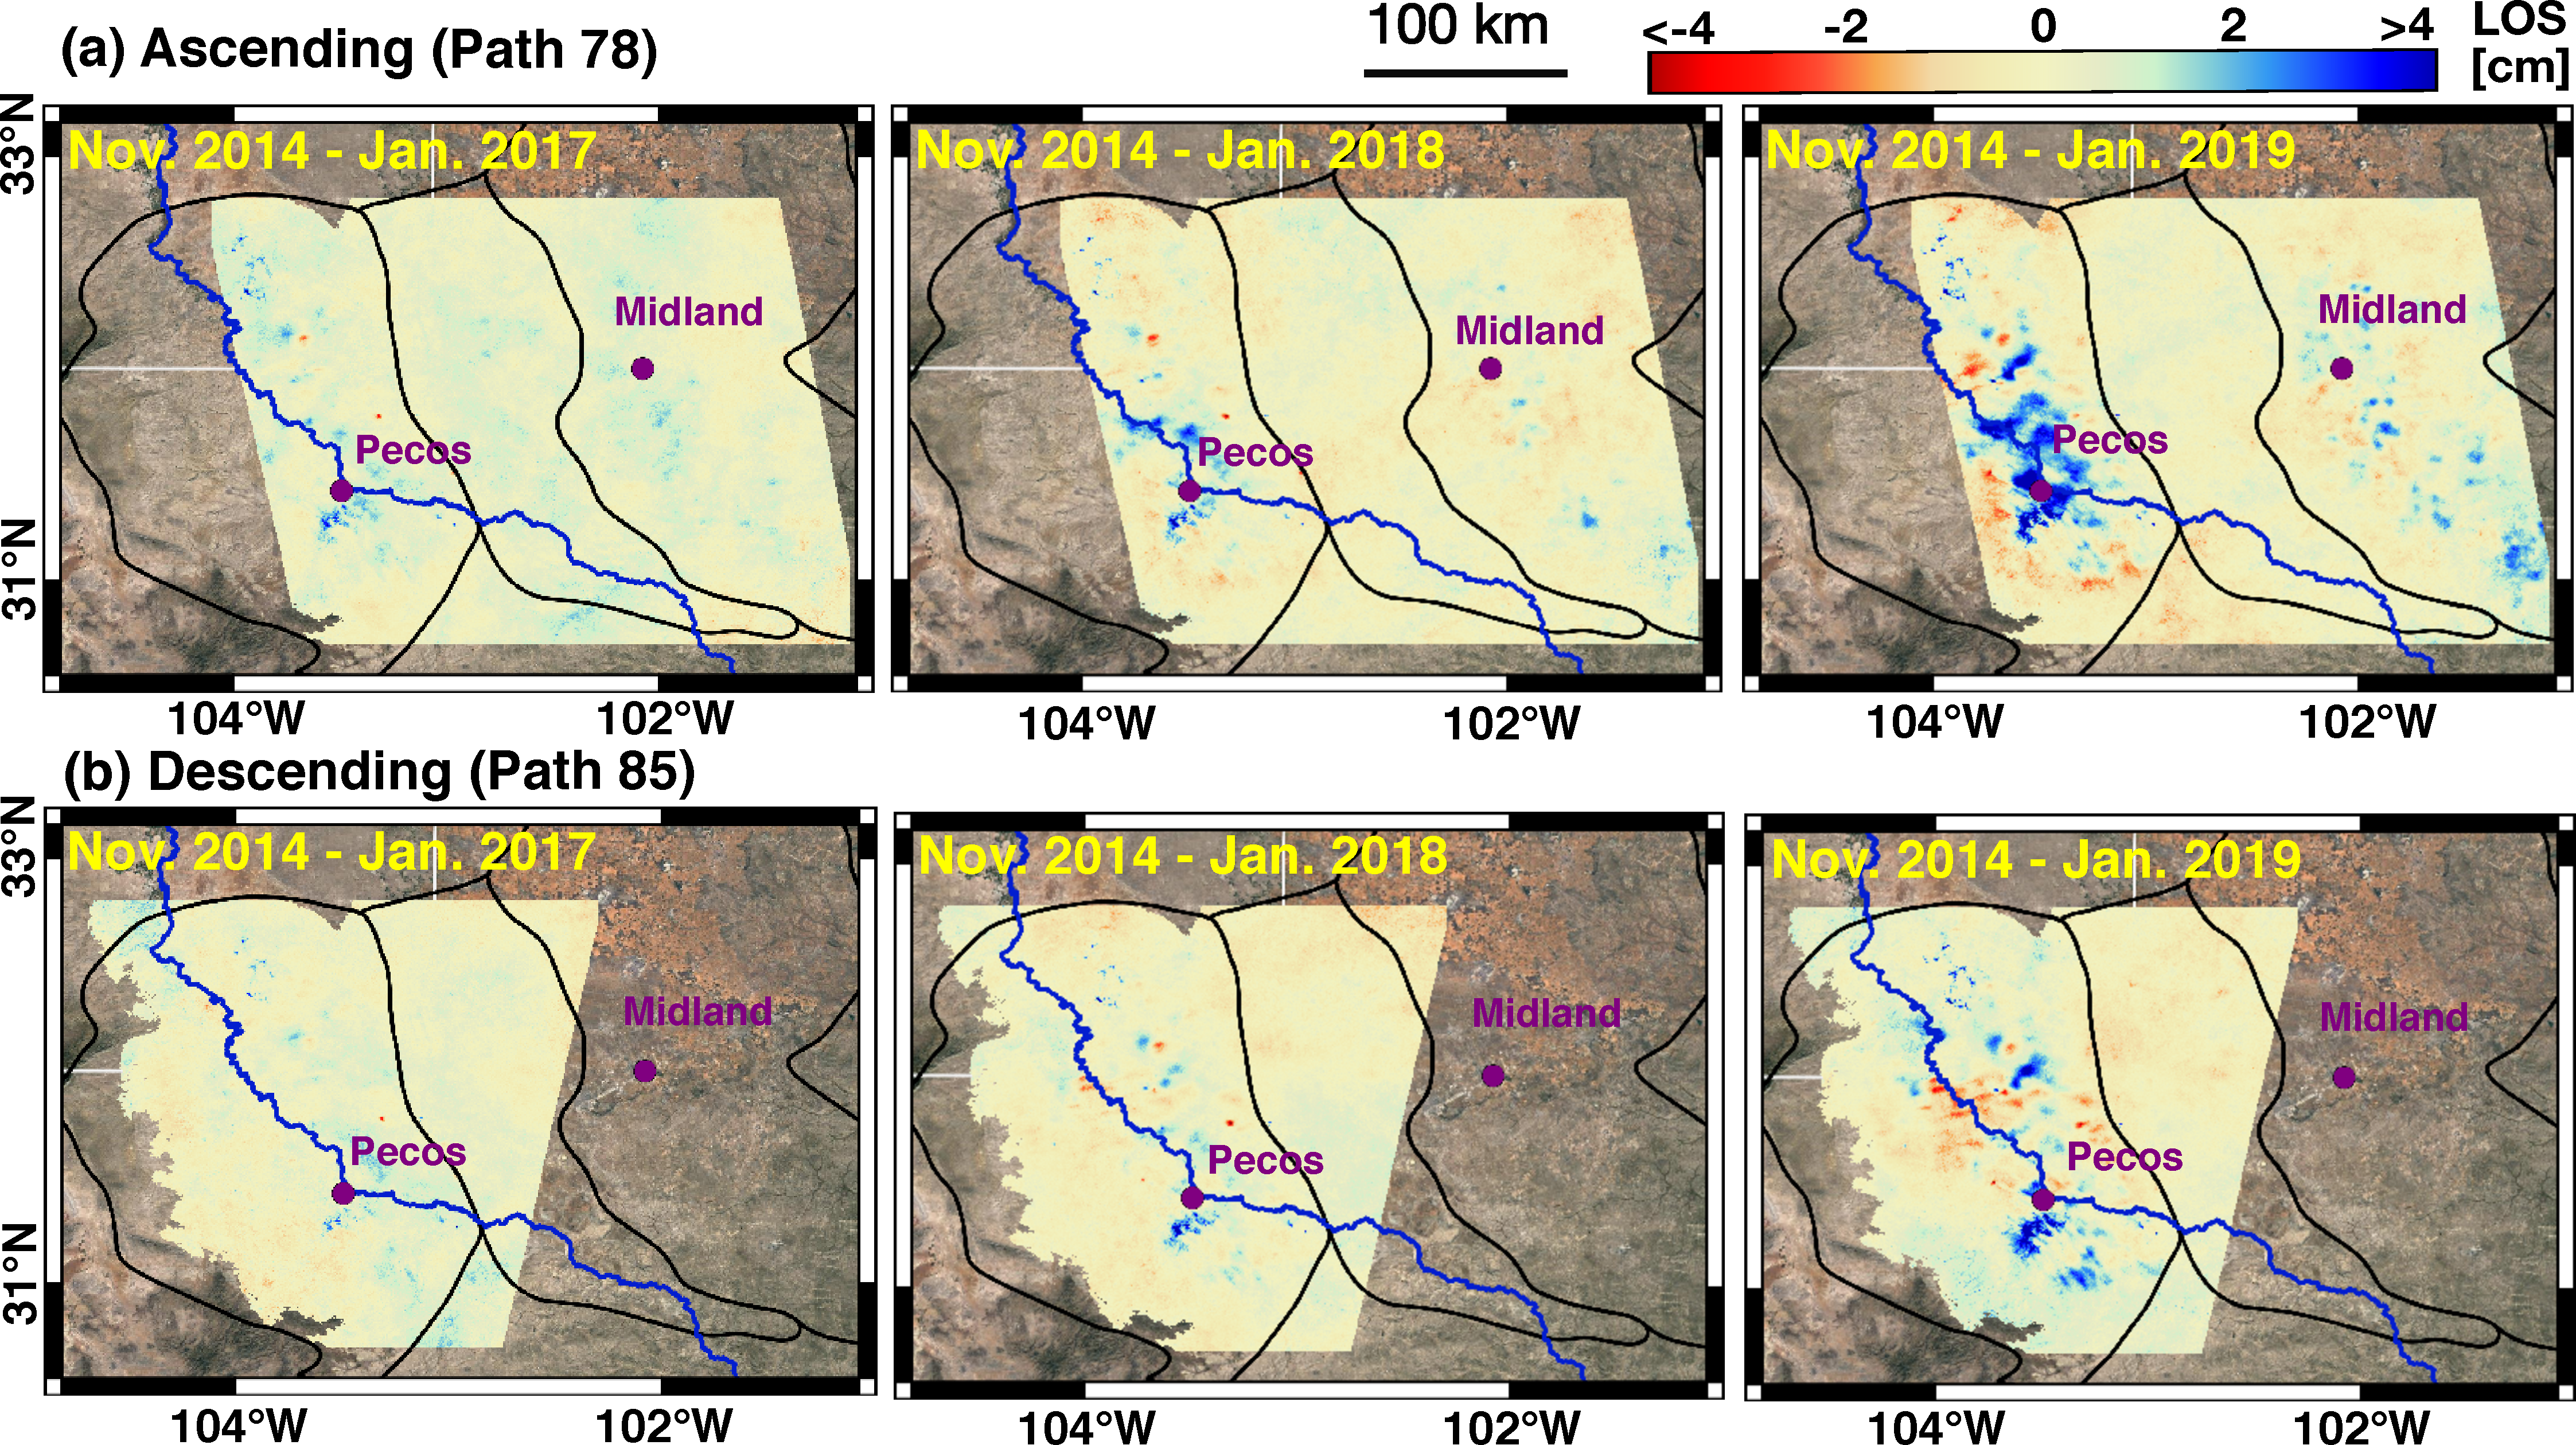
\includegraphics[width=.96\linewidth]{paper1-permian/figures/figure3-los-insar.pdf}
	\caption[Cumulative LOS deformation for path 78 and path 85]{Cumulative LOS deformation (Nov. 2014 - Jan.2017; Nov. 2014 - Jan.2018; Nov. 2014 - Jan. 2019) as inferred from Sentinel-1 (a) ascending path 78, and (b) descending path 85 data over an 80,000 square km oil-producing region of the Permian Basin. Here a subsidence or eastward deformation signal leads to a positive LOS measurement in the ascending geometry, and a subsidence or westward deformation signal leads to a positive LOS measurement in the descending geometry. Areas with $>$1200 m altitude are masked due to the low oil production activity in mountainous regions.}
	\label{fig:insar-los}
\end{figure}

In the northern Delaware Basin, where large volumes of oil production and wastewater disposal occurred, the ascending and descending LOS deformation patterns are similar. This means that the observed deformation in this region is primarily vertical (Figure \ref{fig:insar-decomp} (b) and (e)). The observed subsidence or uplift features between Nov. 2014 and Jan. 2019 are $\sim$ 1-4 cm. In the southern Delaware Basin, \cite{Deng2020SurfaceDeformationInduced} solved for the cumulative LOS surface deformation between Nov. 2014 and Feb. 2019 ($\sim$ 100 km by 60 km) using the ascending Sentinel-1 data (path 78 frames 99-100). In this study, we found that the observed magnitudes of the ascending and descending LOS deformation are different (Figure \ref{fig:insar-los}), which suggests that both horizontal and vertical deformation occurred in this region. Previous studies near Mesquite, Nevada have shown that confined aquifer pumping in the presence of faults can produce complex asymmetrical deformation patterns with a non-trivial horizontal component \citep{Burbey2008InfluenceGeologicStructures}. In the Pecos area, the largest subsidence patterns ($\sim$ 13 cm over 4 years) occurred $\sim$ 15 km south of Pecos, and the largest eastward motion ($\sim$ 3-4 cm over 4 years) occurred near the town of Pecos along a line transect (Figure \ref{fig:insar-decomp} (c) and (f)). The observed linear deformation patterns parallel the inferred favorable fault plane orientation (a strike angle $\sim$ 300 degree lining up with the measured $S_{Hmax}$ direction) proposed by \cite{LundSnee2018StateStressPermian}, and they also align with a cluster of recent shallow earthquakes ($<$ 3 km depth) cataloged by TexNet.



\begin{figure}[hbt!]
	\centering
	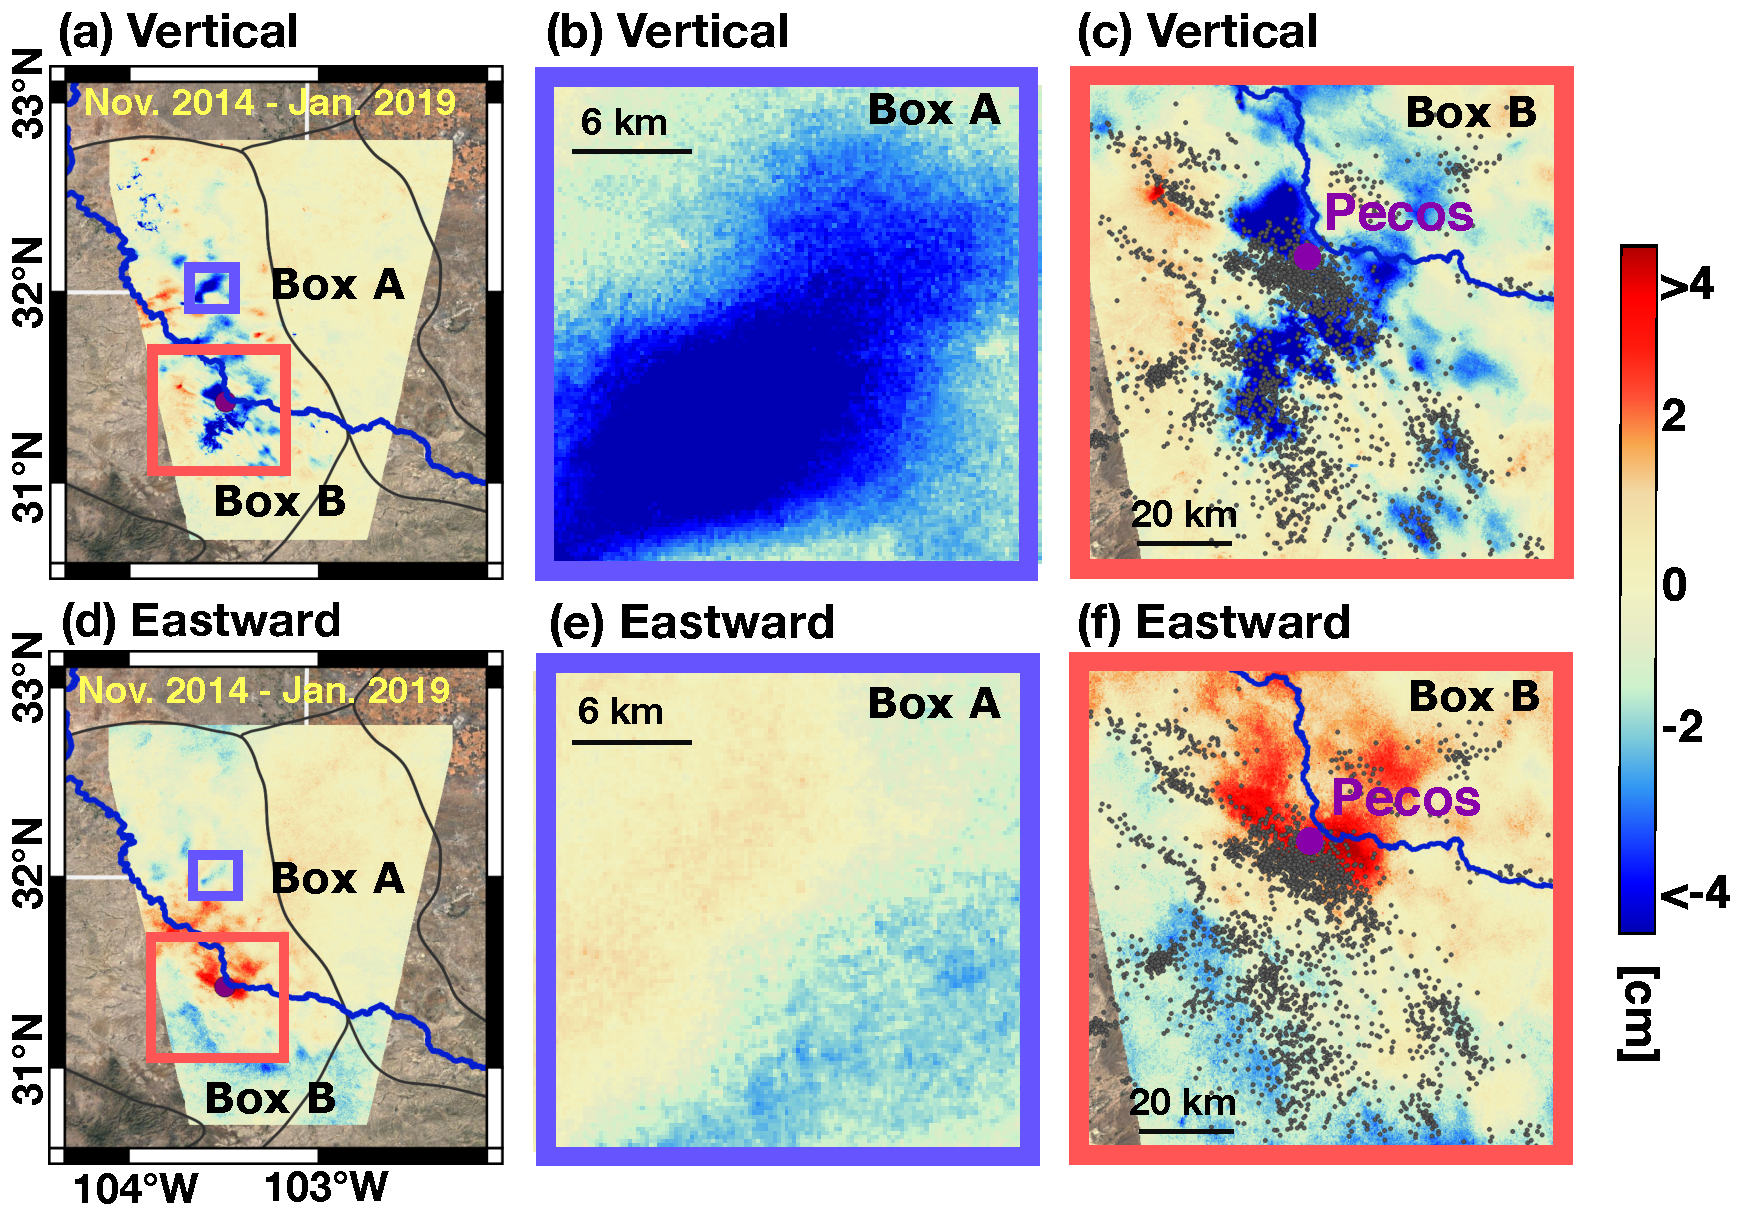
\includegraphics[width=0.96\linewidth]{paper1-permian/figures/figure4-east-vertical-6panel-labelled.pdf}
	\caption[Cumulative vertical and horizontal deformation]{(a) Cumulative vertical deformation between Nov. 2014 and Jan. 2019 over the region where Sentinel-1 path 78 and path 85 overlap. A zoomed-in view of Box A in the northern Delaware Basin and Box B in the southern Delaware Basin are shown in panel (b) and (c) respectively. (d) Cumulative eastward deformation between Nov. 2014 and Jan. 2019 over the region where Sentinel-1 path 78 and path 85 overlap. A zoomed-in view of Box A in the northern Delaware Basin and Box B in the southern Delaware Basin are shown in panel (e) and (f) respectively. In the southern Delaware Basin, the observed vertical and eastward deformation (panel (c) and (f)) show linear patterns along with earthquake hypocenters (gray dots) detected by TexNet in 2018.}
	\label{fig:insar-decomp}
\end{figure}


\subsection{Implications for geomechanical modeling}
Based on fault plane solutions derived from recent seismic activity and the faulting stress regime interpretations \citep{LundSnee2018StateStressPermian}, the Pecos area is in a normal faulting regime. We employed an elastic dislocation model \citep{Okada1992InternalDeformationDue} to demonstrate that the presence of dip-slip normal faults can produce the observed linear subsidence patterns in this area (Figure \ref{fig:model} (a)). We solved for the dip angle, depth, width along the dip direction, and slip magnitude of four normal faults by best fitting the forward model to InSAR vertical deformation observations, minimizing the sum of squared residuals, and maximizing the r-squared values \citep{Du1992ComparisonVariousInversion} (Appendix \ref{appen:okada}). The optimal solution suggests that the depth of the faults ranges from 0.9 km to 1.5 km, which is shallower than most of the TexNet recorded earthquakes (2-6 km in depth). Possible explanations for this discrepancy include: (1) the existence of aseismic fault slippage being responsible for the observed surface deformation \citep{McGarr2017WastewaterDisposalEarthquake}; (2) bias in earthquake depth estimation in the TexNet catalog \citep{Lomax2019ImprovingAbsoluteEarthquake}; (3) systematic modeling errors associated with representing a mechanically layered earth as a homogeneous half space \citep{Du1992ComparisonVariousInversion}. 



\begin{figure}[hbt!]
	\centering
	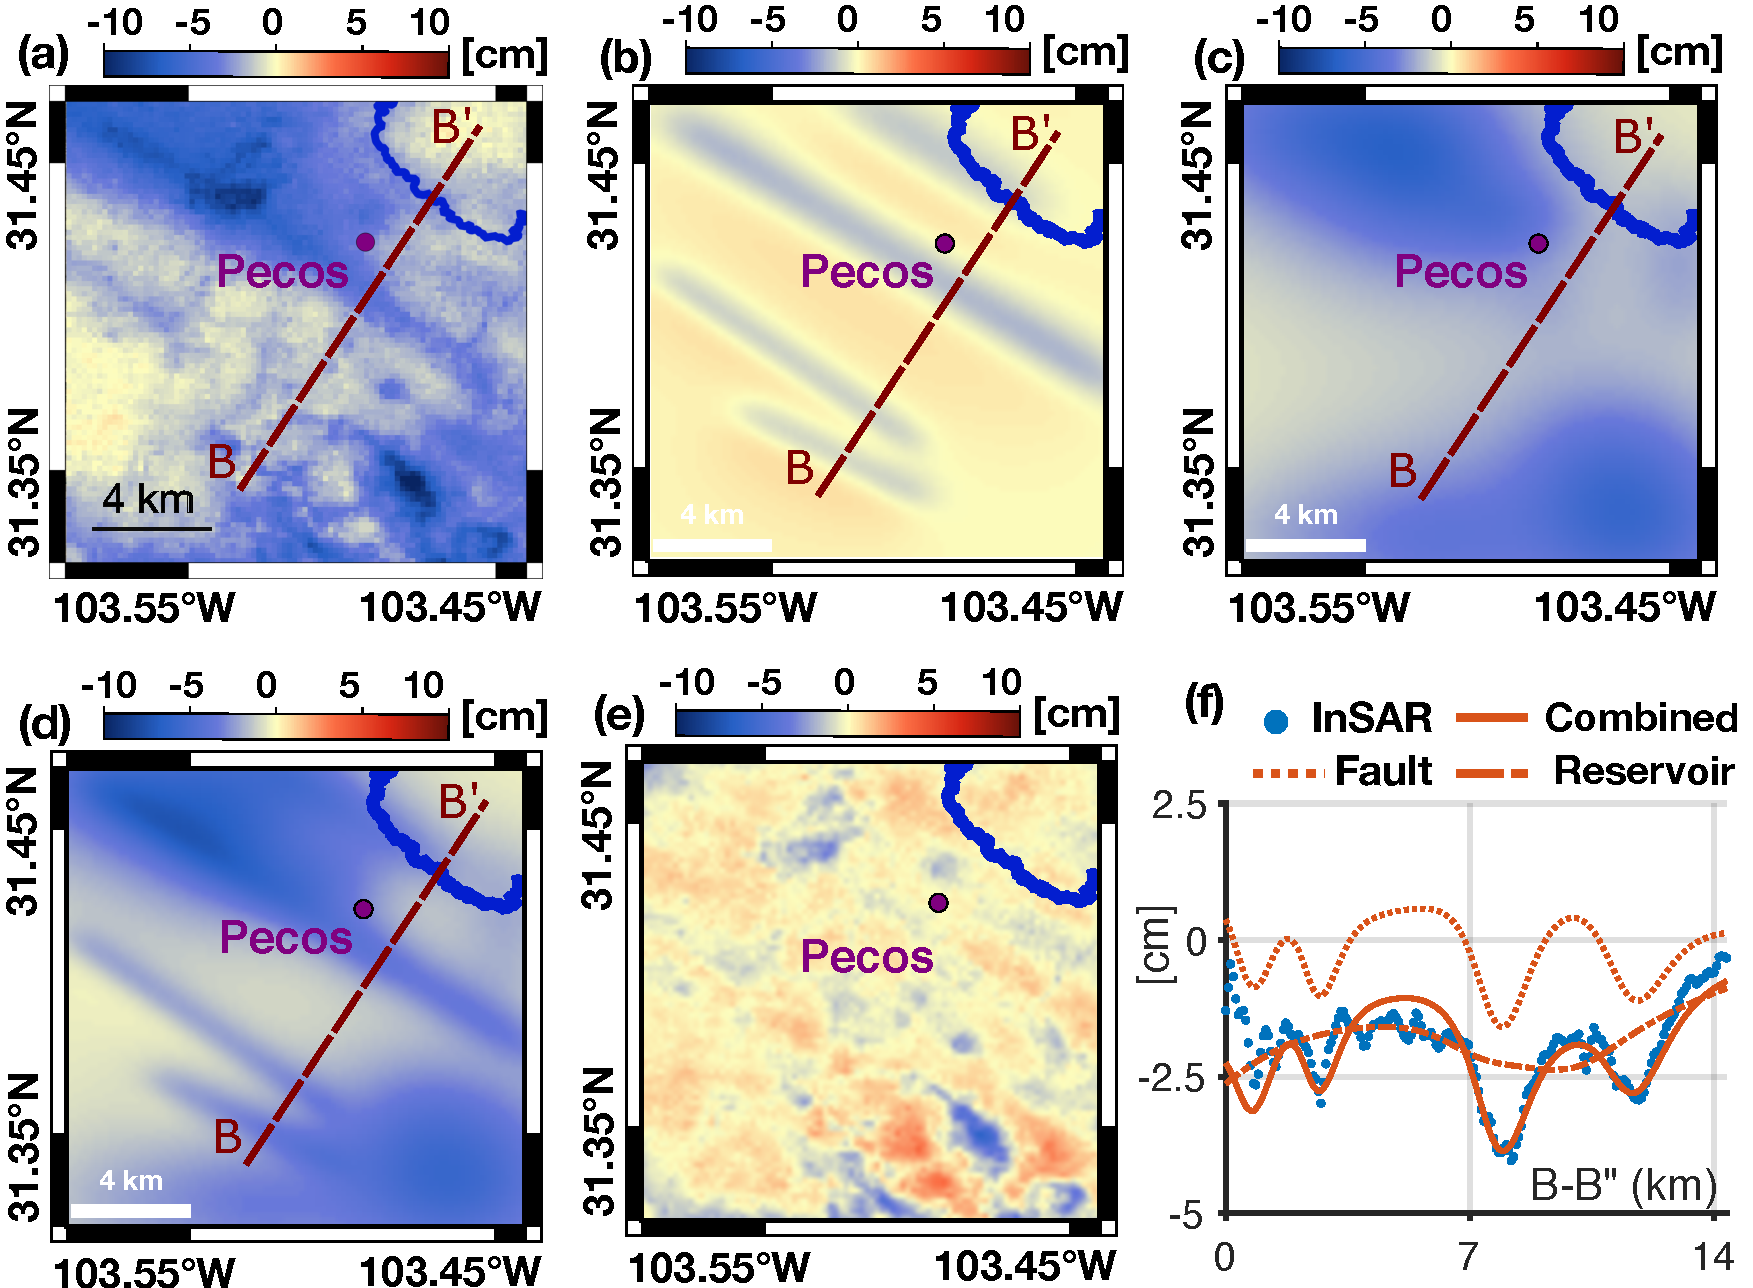
\includegraphics[width=\linewidth]{paper1-permian/figures/figure5-modeling.pdf}
	\caption[Modeled surface deformation from fault slip and reservoir subsidence]{(a) InSAR-observed cumulative vertical deformation between Nov. 2014 and Jan. 2019 in the Pecos, TX area. (b) Modeled vertical deformation associated with four dip-slip faults. (c) Modeled vertical deformation associated with reservoir compaction. (d) Modeled total vertical deformation associated with four dip-slip faults and reservoir compaction (panel (b) $+$ panel (c)). (e) Difference between InSAR-observed and model-predicted vertical deformation (panel (a) $-$ panel (d)). (f) Difference between InSAR-observed and model-predicted vertical deformation along the B-B' transect.}
	\label{fig:model}
\end{figure}


After removing the best-fit deformation associated with dip-slip faulting (Figure \ref{fig:model} (b)), there is still $\sim$ 2 cm residual subsidence in the Pecos area (e.g. Figure \ref{fig:model} (f)). Given that shallow groundwater production was minimal in this region for the time period of interest \citep{Deng2020SurfaceDeformationInduced}, we introduced an elastic reservoir compaction model \cite{Geertsma1973LandSubsidenceCompacting} to our geomechanical analysis (Appendix \ref{appen:model-compact}). We implemented two layers of multiple cylindrical reservoirs corresponding to reported locations and depths of well clusters in the Delaware Mountain Group (DMG) and Wolfcamp reservoirs, which account for most of the recent oil and gas production in the region. We discretized the DMG layer based on a cluster of production wells predominantly perforated over a depth range of 1.5-1.8 km. The Wolfcamp wells are completed over a depth range of 3-3.6 km. We employed an objective function inversion method to solve for the reservoir pressure depletion pattern that best fit the InSAR-observed subsidence (Figure \ref{fig:model} (c)) \citep{Du2001PoroelasticReservoirModel}.

An important conclusion of this study is that both fault slip and reservoir inflation or compaction can produce observable surface deformation over an 80,000 square kilometer oil-producing region of the Permian Basin. The InSAR-observed subsidence patterns over the Pecos area can be modeled as slip over multiple faults and discretized cylindrical reservoir compaction (Figure \ref{fig:model} (d)-(f)). We note that InSAR subsidence data alone can constrain all pertinent fault and reservoir parameters in our normal faulting and reservoir compaction models. The InSAR observed cumulative surface deformation patterns, which show larger horizontal component than the model prediction, suggest that other factors, such as strike-slip faulting and heterogeneity in subsurface properties, may play a role. There have been extensive studies on how reservoir compaction and inflation as well as fault slippage alter stress fields in the subsurface and produce surface deformation \citep{Geertsma1973LandSubsidenceCompacting,Segall1992InducedStressesDue,Okada1992InternalDeformationDue,Du1992ComparisonVariousInversion,Vasco2005UseQuasiStatic,Vasco2008ReservoirMonitoringCharacterization,Khakim2012GeomechanicalModelingInsar}. InSAR surface deformation can be combined with this knowledge to evaluate fluid recovery efficiency and monitor disposal wells at low cost. Furthermore, these high-quality geodetic measurements are readily available to complement the TexNet seismic catalog for assessing the likelihood of fault motion and induced earthquake risks in Texas.


